\documentclass[tikz,border=4pt]{standalone}
\usepackage{amsmath,amssymb}
\usetikzlibrary{arrows.meta}
\begin{document}
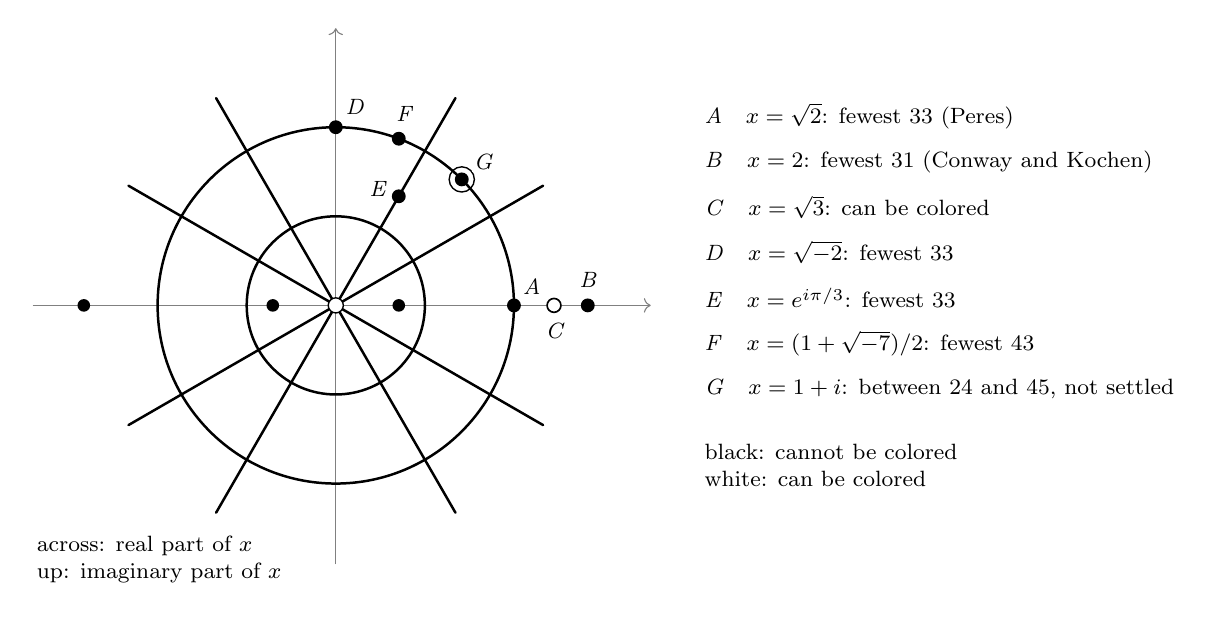
\begin{tikzpicture}[line cap=round,line join=round]
\begin{scope}[scale=1.6]
\draw[->,gray] (-2.4,0) -- (2.5,0);
\node[font=\footnotesize,anchor=north west] at (-2.45,-1.75) {across: real part of $x$};
\draw[->,gray] (0,-2.05) -- (0,2.2);
\node[font=\footnotesize,anchor=north west] at (-2.45,-1.97) {up: imaginary part of $x$};
\foreach \t in {30,60,120,150} \draw[line width=0.9pt] (\t:-1.9) -- (\t:1.9);
\draw[line width=0.9pt] (0,0) circle (1.4142);
\draw[line width=0.9pt] (0,0) circle (0.7071);
\foreach \p in {-2,-0.5,0.5,2} \fill (\p,0) circle (0.05);
\draw[fill=white,line width=0.5pt] (0,0) circle (0.06);
\fill (1.4142,0.0000) circle (0.055);
\node[font=\footnotesize\itshape,fill=white,inner sep=0.8pt] at (1.5542,0.1500) {A};
\node[right,font=\footnotesize] at (2.85,1.5000) {\textit{A}\quad $x=\sqrt2$: fewest 33 (Peres)};
\fill (2.0000,0.0000) circle (0.055);
\node[font=\footnotesize\itshape,fill=white,inner sep=0.8pt] at (2.0000,0.2000) {B};
\node[right,font=\footnotesize] at (2.85,1.1400) {\textit{B}\quad $x=2$: fewest 31 (Conway and Kochen)};
\draw[fill=white,line width=0.6pt] (1.7321,0.0000) circle (0.055);
\node[font=\footnotesize\itshape,fill=white,inner sep=0.8pt] at (1.7321,-0.2000) {C};
\node[right,font=\footnotesize] at (2.85,0.7800) {\textit{C}\quad $x=\sqrt3$: can be colored};
\fill (0.0000,1.4142) circle (0.055);
\node[font=\footnotesize\itshape,fill=white,inner sep=0.8pt] at (0.1500,1.5742) {D};
\node[right,font=\footnotesize] at (2.85,0.4200) {\textit{D}\quad $x=\sqrt{-2}$: fewest 33};
\fill (0.5000,0.8660) circle (0.055);
\node[font=\footnotesize\itshape,fill=white,inner sep=0.8pt] at (0.3300,0.9260) {E};
\node[right,font=\footnotesize] at (2.85,0.0600) {\textit{E}\quad $x=e^{i\pi/3}$: fewest 33};
\fill (0.5000,1.3229) circle (0.055);
\node[font=\footnotesize\itshape,fill=white,inner sep=0.8pt] at (0.5400,1.5229) {F};
\node[right,font=\footnotesize] at (2.85,-0.3000) {\textit{F}\quad $x=(1+\sqrt{-7})/2$: fewest 43};
\fill (1.0000,1.0000) circle (0.055);
\draw[line width=0.5pt] (1.0000,1.0000) circle (0.1);
\node[font=\footnotesize\itshape,fill=white,inner sep=0.8pt] at (1.1700,1.1400) {G};
\node[right,font=\footnotesize] at (2.85,-0.6600) {\textit{G}\quad $x=1+i$: between 24 and 45, not settled};
\node[right,font=\footnotesize,align=left] at (2.85,-1.2700) {black: cannot be colored\\white: can be colored};
\end{scope}
\end{tikzpicture}
\end{document}
